

\documentclass[a4paper, 12pt]{report} 

\usepackage[utf8]{inputenc}  
\usepackage{amsmath, amssymb}   
\usepackage{graphicx} 
\usepackage{hyperref}  

\title{Simple Report Example}
\author{Hemanth S.P}  
\date{\today}  

\begin{document}

\maketitle  

\tableofcontents  

\chapter{Introduction}  
This is the introduction of the report. In this report, we discuss several concepts, such as \LaTeX\ formatting and document structuring.

\section{Background}  
This section provides background information about the report's topic.

\subsection{History of LaTeX}  
LaTeX was created by Leslie Lamport in the early 1980s as a document preparation system based on Donald Knuth's TeX typesetting system.

\chapter{Methodology}  
In this chapter, we describe the methods and techniques used to accomplish the research presented in this report.

\section{Research Method}  
The research method used is a combination of quantitative and qualitative approaches.

\chapter{Results and Discussion} 
This chapter discusses the findings from the research, including charts, figures, and tables.

\section{Graphical Representation}  
Below is a simple graphical representation:

\begin{figure}[h]  
\centering
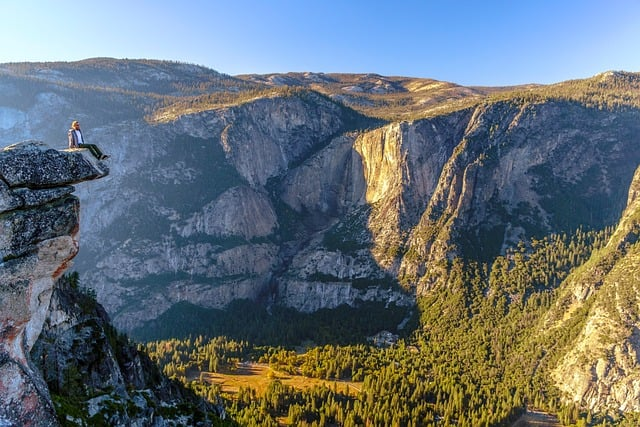
\includegraphics[width=0.5\textwidth]{image2.jpg}  
\caption{Example of a Graph}
\end{figure}

\chapter{Conclusion} 
In this report, we have presented several concepts. The conclusion summarizes the findings and discusses future work.

\end{document}
